\section{Introduction}
Fork-based development allows developers to start development from existing software repository by copying the code files, and gives developers the freedom and independence to make modifications on their own fork~\cite{dubinsky2013exploratory, bitzer2006impact, ernst2010code,vetter2007open}, and it has been widely used in both open source communities and industries. But when the number of forks grows, it becomes difficult to keep track of decentralized development activity in many forks. Some of the developers on Github we have interviewed previously confirmed the problems they faced in terms of losing overview of forks. For example, one said: \emph{"I do not have much visibility of the forks. They are too many and it is overwhelming to keep track of them"} ~\cite{ZSLXWK:ICSE18}. Both Duc et al. and Berger et al. found that this problem also appears in industrial that it?s hard for individual teams to know who is doing what and what code changes are made in other forks~\cite{berger2014three,Duc:2014:FCM:2652524.2652546}.

Even though GitHub supports a network view and member view, it is difficult to gain a straightforward overview of specific activities in forks. As another developer said: \emph{"The network view is helpful for seeing how active a fork is, but often you have to scroll back a lot to find the fork point and then you have to go to the end again for seeing what changed since then in the parent and in the fork, by reading the tooltips of each commit. And the Members view is just a big list of projects, only helpful for finding the parent of all forks, and for opening all of them in browser tabs to read the descriptions."}\Luyao{Should I fix typos in quota?} \footnote{\url{https://github.com/dear-github/dear-github/issues/175}}
 A lack of an overview of forks leads to several additional problems: 1) redundant development: developers may re-implement functionality has already been developed elsewhere; 2) lost contributions: the contributions developers made are easily lost to the larger community unless they contribute those changes back to the original project; 3) suboptimal forking point: developers might not fork from the codebase that is closest to their intended goals ~\cite{ZSLXWK:ICSE18, dubinsky2013exploratory,stanciulescu2015forked}. So it's necessary to give developers a panoramic view to help them better understand activities among various forks.

Forks Insight\footnote{\url{http://www.forks-insight.com}} is a product of academic technology transfer based on the idea of INFOX \cite{ZSLXWK:ICSE18}. We are trying to make those research results more accessible to practitioners. Comparing to INFOX, Forks Insight is more light-weighted and has no limit to programming language. It provides an overview of each repository in fork-level granularity, and deliver insights to interested developers including repository's maintainers and ac-hoc developers who are interested in the repositories and want to see others' secondary development, and potentially eliminate the problems that we mentioned before.

\todo[inline]{related work}

\section{Forks Insight}

Forks Insight is aiming for providing facilities to explore unintegrated changes to find opportunities for reuse, to find inspirations for further development, to connect developers working on similar topics.
%
The same as INFOX did, Forks Insight analyzes each active fork of a repository and takes the diff between the fork point and the latest commits \todo{need to check}  of the fork and extracting keywords from code changes, comments and commit messages.
%
Besides, Forks Insight presents statistical data of code changes in the granularity of commit, file and line. The user interface of Forks Insight is shown in Fig.~\ref{GUI}. 

Users could login with their own GitHub accounts, and subscribe repositories on GitHub by importing from their public repositories or search for repository url. Forks Insight will start crawling and analyzing data if the repository is not in the database yet and remind the user when it's finished.

\begin{figure}[t]
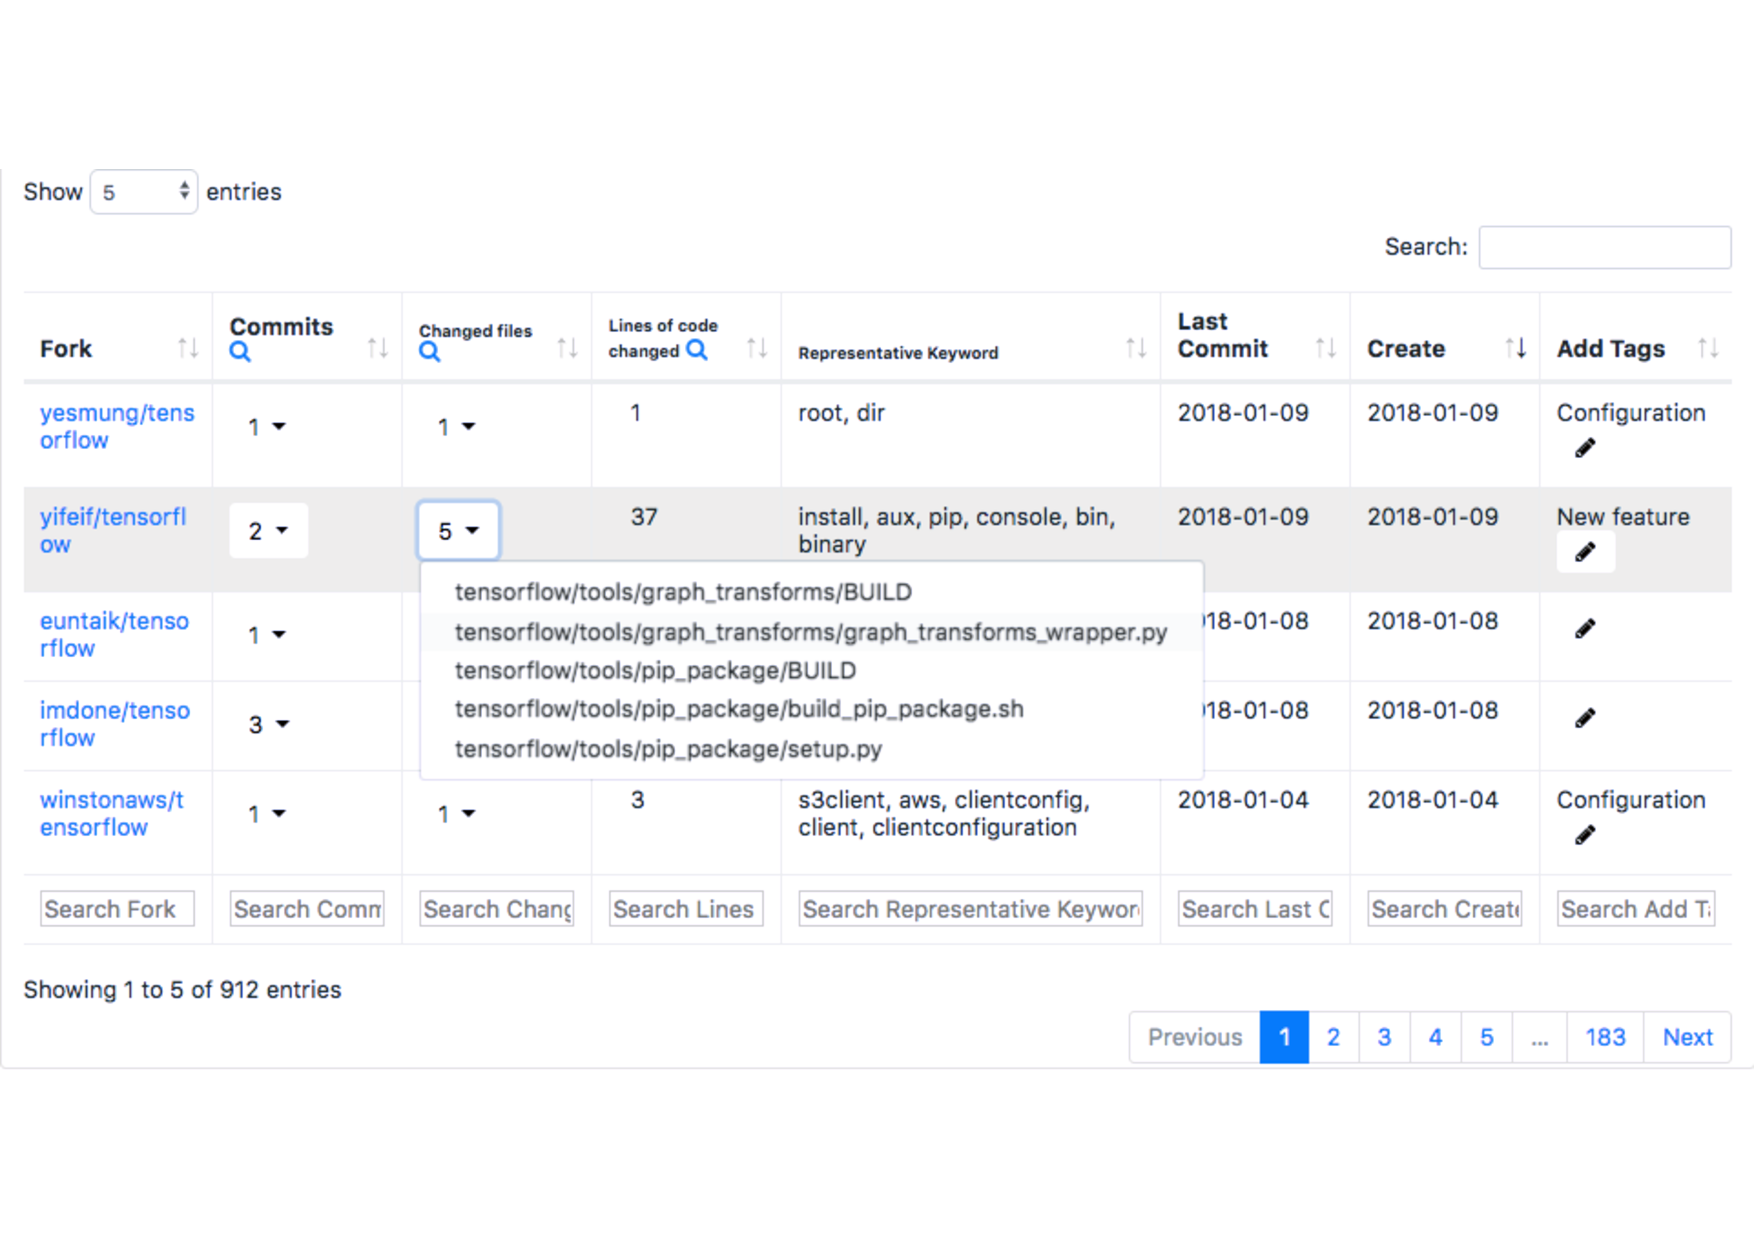
\includegraphics[scale=0.3]{tensorflow_snapshot4.pdf}
\caption{User Interface of Forks Insight.\Luyao{(TODO)add arrows as poster did?}}
	\vspace{-15pt}
	 \label{GUI}
\end{figure}

\subsection{Extracting Keywords}
As for the column of representative keywords, we use well-known natural language processing technique TF-IDF \cite{salton1988term} on text related to code changes, such as source code, comments, and corresponding commit messages. First, we do some preprocessing: remove all the numeric strings; split for underline-separated and Camel-Case cases; lemmatize words to a normal form. Second, we use TF-IDF technique to extract keywords from the text. Though TF-IDF can effectively filter some stop words like "or", "and", there are still some words with high weight like "public", "private" which is common in language like Java/C++. To improve our result, we manually added the stop words list for different programming language corresponding to their different characteristics.
%
Fortunately, our method runs fast and has no limit for repository's programming language. Forks Insight can successfully analyze the most popular repositories on Github in hours for the first time.

\subsection{Tagging}
Developers fork a repository for different reasons: adding new features, fixing bugs, and changing configuration, etc.~\cite{Mikkonen2011,Robles2012,dubinsky2013exploratory,stanciulescu2015forked}.
%
Since tagging is a simple and intuitive way to summarize the purpose of forking and also convenient to cluster similar forks. So we add a column at the end of each row to allow user to annotate the tags manually on forks. We hope user's contribution on tags can not only help themselves maintain and understand each fork which may reduce the redundant development, but also help the whole open source community, especially for the new users who are interested in this repository but not familiar with repositories. The data of tagging will also be useful for future research work.

\Shurui{Fork Insight allows users to tag each fork by the main activity of each fork based on their understanding. This data could help users to manage and classify forks with similar goals.}

\subsection{Searching}

\begin{figure}[]
\centering
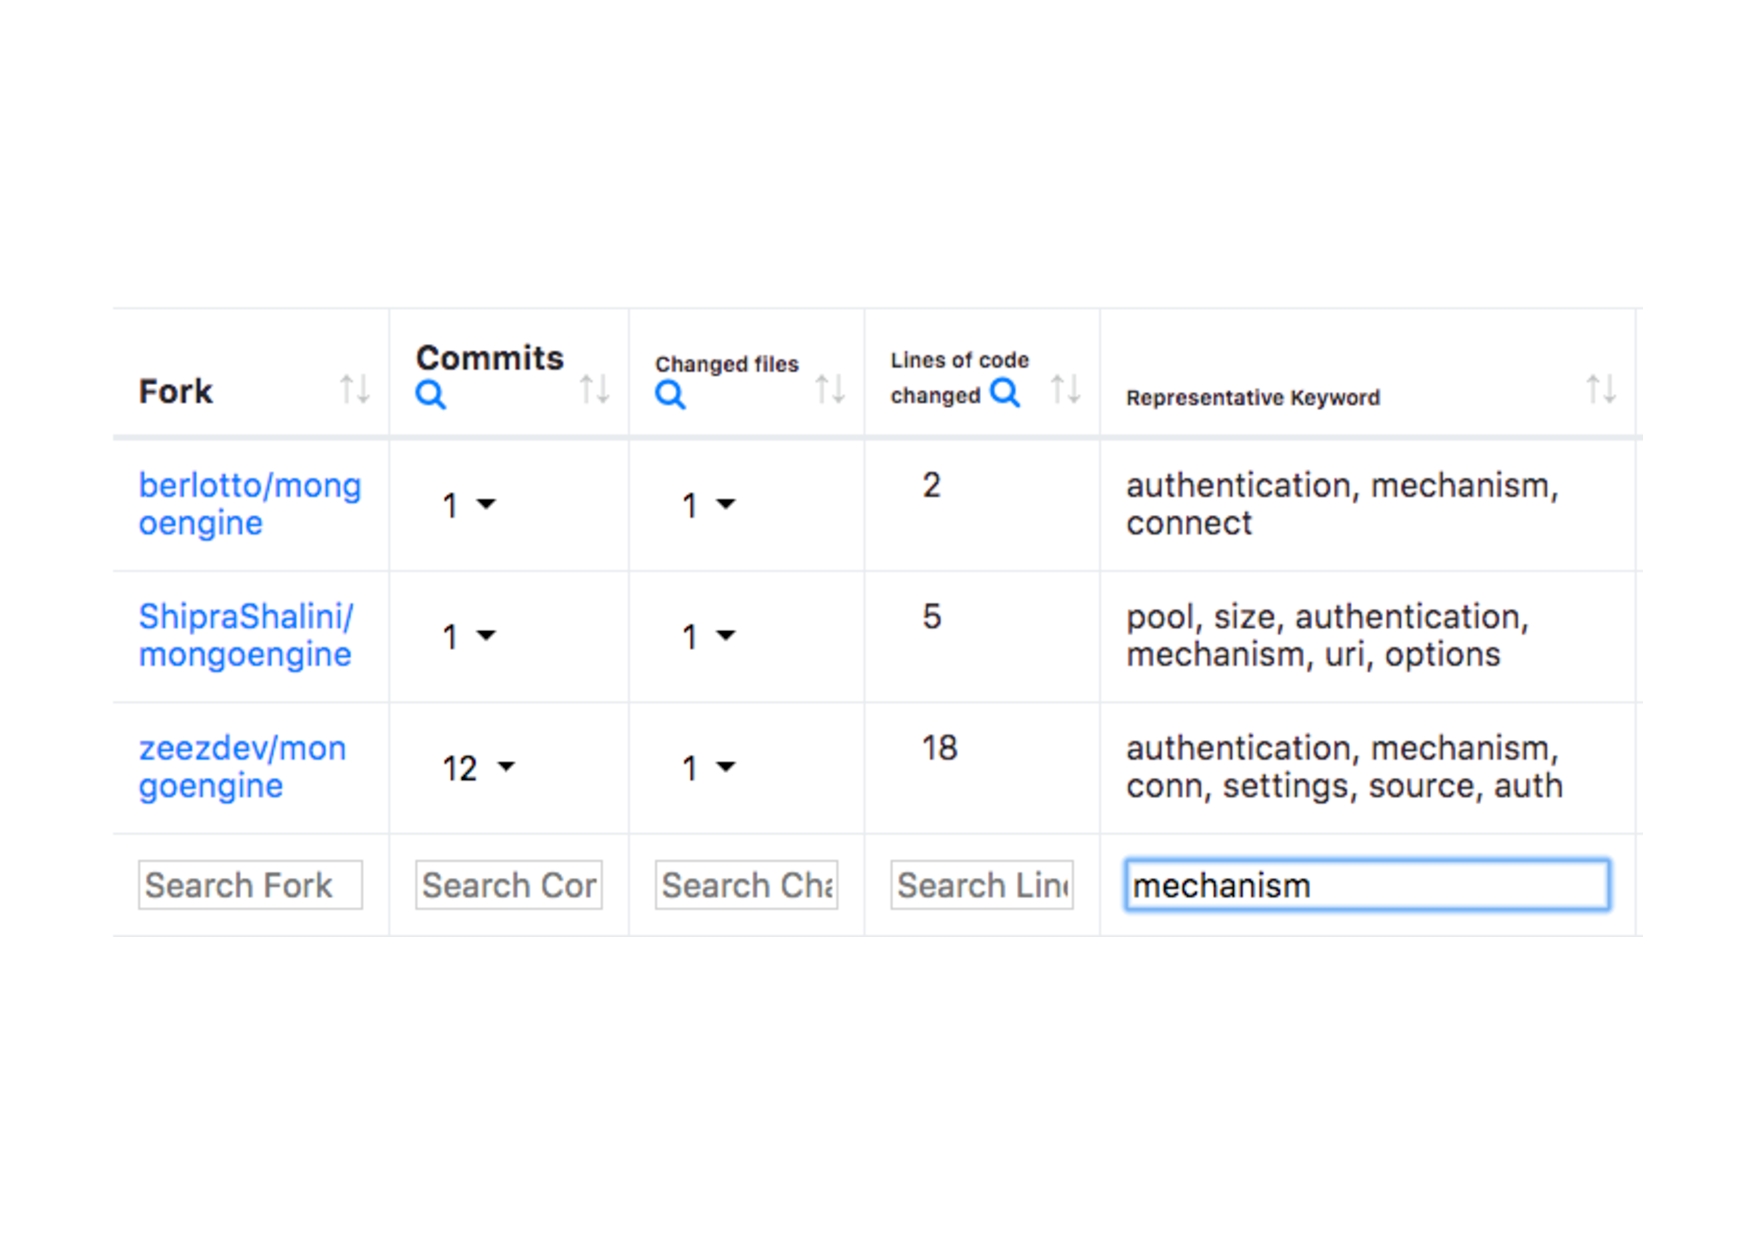
\includegraphics[scale=0.3]{pic5.pdf}
\caption{An example of searching for similar forks.}
\vspace{-12pt}
\end{figure}
Forks Insight also supports searching forks by keywords. For example, in Fig. 2, searching for "mechanism" in forks of MongoEngine\footnote{\url{http://www.forks-insight.com/project/MongoEngine/mongoengine}}, will get three forks which are all related to "mechanism of authentication during connection with database", and contain the same changed file. The example shows that by using keyword search in Forks Insight, user could find out some similar forks that could probably cut down the possibility of the redundant development.

\section{Conclusions and Future Work}
We implemented a tool to help developers get an overview of forks. The current release version focuses on simple analytics for the high level overview which is lightweight, scalable and practical. In order to improve the usability of Forks Insight, we plan to design a user study. And we would like to add more interactive elements and powerful functions into our tool. There are several directions we are considering to move forward: using more visualization to show the meaningful data; identifying features in forks; summarizing the activities of forks by natural language.

\begin{acks}
  TODO
\end{acks}


